\documentclass[tikz]{standalone}
\usepackage{tkz-euclide}
\begin{document}
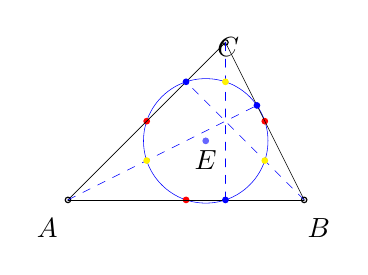
\begin{tikzpicture}
    \tkzDefPoints{0/0/A,3/0/B,2/2/C}
    \tkzDefCircle[euler](A,B,C) \tkzGetPoints{E}{e}
    \tkzDrawCircle[blue](E,e)
    \tkzDefMidPoint(A,B) \tkzGetPoint{M_c}
    \tkzDefMidPoint(A,C) \tkzGetPoint{M_b}
    \tkzDefMidPoint(B,C) \tkzGetPoint{M_a}
    \tkzDrawPoints(A,B,C) \tkzDrawPoints[blue!60](E)
    \tkzDrawPoints[red](M_a,M_b,M_c)
    \tkzDrawSegments(A,B B,C A,C)
    \tkzLabelPoints(E)
    \tkzAutoLabelPoints[center=E](A,B,C)
    \tkzDefPointBy[projection=onto A--B](C) \tkzGetPoint{H_c}
    \tkzDefPointBy[projection=onto B--C](A) \tkzGetPoint{H_a}
    \tkzDefPointBy[projection=onto A--C](B) \tkzGetPoint{H_b}
    \tkzDrawPoints[blue](H_a,H_b,H_c)
    \tkzDrawSegments[blue,dashed](A,H_a B,H_b C,H_c)
    \tkzDefTriangleCenter[ortho](A,B,C) \tkzGetPoint{H}
    \tkzDefMidPoint(A,H) \tkzGetPoint{E_a}
    \tkzDefMidPoint(B,H) \tkzGetPoint{E_b}
    \tkzDefMidPoint(C,H) \tkzGetPoint{E_c}
    \tkzDrawPoints[yellow](E_a,E_b,E_c)
\end{tikzpicture}
\end{document}